\documentclass[11pt,twocolumn]{article}
\usepackage{graphicx}
\usepackage[margin=1in]{geometry}
\usepackage{natbib}
\usepackage{amsmath, amssymb, graphicx}
\usepackage{authblk}
\usepackage{url}
\usepackage{setspace}

\renewcommand\Authfont{\normalsize}
\renewcommand\Affilfont{\small}
\setlength{\affilsep}{0pt}

\providecommand{\apj}{ApJ}
\providecommand{\apjl}{ApJL}
\providecommand{\apjs}{ApJS}
\providecommand{\aap}{A\&A}
\providecommand{\mnras}{MNRAS}
\providecommand{\na}{New Astronomy}
\providecommand{\nat}{Nature}
\providecommand{\jaavso}{JAAVSO}
\providecommand{\aj}{AJ}
\providecommand{\araa}{ARA\&A}
\providecommand{\pasp}{PASP}

\begin{document}

\title{\textbf{T-Mobile Park's Effect on \\ Major League Baseball in Seattle}}
\author{Brodie Monohan}
\affil{\textit{University of Washington}}
\affil{monohanb@uw.edu}

\date{August 7, 2026}

\twocolumn[
\begin{@twocolumnfalse}
\maketitle

\begin{abstract}
The Seattle Mariners are the only Major League Baseball team to never appear in a World Series. Despite being near the middle of the pack in terms of payroll, Mariner teams since the early 2000s have been disappointing to say the least, with historically bad offenses in the 2010s. Since the team's move from their old stadium into what would become T-mobile Park (formerly Safeco Field), some analysts have noticed that batters seem to perform poorly in the stadium. Former sluggers who were traded to the Mariners would constantly under-perform with their new team, or so it seemed. Some analysts began to theorize there was some external factor causing batters to lose production when being traded to the Mariners. The most prominent theory is that the Seattle climate and the stadium itself that was causing hitters to under-perform. This theory is reinforced by the pitching statistics for Seattle which, since 2000, have been historically good. While a ``cursed'' stadium is a romantic way to explain the Mariner's historic woes, there is also a much more ordinary explanation: that Mariners have just been bad hitters. This project examines if hitting in Seattle is significantly ``harder'' or if players are worse when playing in Seattle by looking at historical batting numbers and investigating the physical conditions of T-Mobile Park.
\end{abstract}

\vspace{1cm}
\end{@twocolumnfalse}
]

\doublespacing

\section{Research Questions}
I set out to answer three quesitons about the supposed disadvantages for hitters in T-Mobile Park. The first quesiton was whether hitter performance demonstrated a systematic hinderance as a Seattle Mariner or at T-Mobile Park by looking at traded player performance and historic home vs away splits respectively. The results indicate no systematic trends in loss of production as a Seattle Mariner or in T-Mobile Park. Average change in performance remained within \_\_ of zero for both home/away splits and season performce on either side of a trade with Seattle for a range of stats including On-Base Percentage (OBP), Slugging Rate (SLG), Home Run rate (HR rate), hits, and Batting Average (BA, home/away only). The second question was whether the enviromnent of T-Mobile Park (and Seattle in general) where significant factors on the flight of a baseball such that playing at T-Mobile Park is significantly disadvantageous in terms of how far a ball travels for given hit parameters. The results did show a significant difference in trajectories between stadiums. Based on temperature, elevation, and coordinate data, a ball hit in the range of typical home-run parameters can travel up to 10 meters farther in Colorado compared to Seattle. The third question was if these results indicated an overall competitive disadvantage for the Seattle Mariners. The results for this question were mixed. Historical slugging numbers suggest that Mariner teams, especially in the past few years, have relied on hard-hit balls, slugging, and homeruns which the above questions showed mixed results on. The first question indicated that historically, SLG and HR rate were seemingly unaffected by T-Mobile Park or the Mariners organization, however, the second question indicated that there is a physical limitation in T-Mobile Park for hard-hit and high hang-time balls, like home-runs. Possible explainations are explored in the results section.

\section{Motivation}
My motivation for this research has stayed pretty much the same which is described in the abstract (I put it up there becuase I think it is better to read first and it goes nicely into a README). I wanted to investigate the ad nauseum argument that hitting is harder in Seattle. I made no updates since the EDA assignment.

\section{Dataset(s)}
My main dataset comes from \texttt{pybaseball}. The MLB and third parties have tracked statistics since far before the 1999 season when the Mariners changed stadiums, however, the MLB started to take advanced statistics after the 2014 season with StatCast which includes things like swing speed, launch angle, launch velocity, and other advanced metrics which will be useful for my analysis. An open source Python package already exists for these analytics called \texttt{pybaseball} which scrapes Baseball Savant (built on StatCast), as well as Baseball Reference which are two more proprietary baseball statistic trackers. Documentation can be found at \url{pypi.org/project/pybaseball/}. This package works with \texttt{pandas} and can be indexed and manipulated as a DataFrame.

My second dataset comes from \texttt{open-mateo}. 


\section{Method}

\subsection{Historical Batting}

I look at systematic drops in batter performance in T-Mobile Park by comparing home and away splits as well as season perfromace on either side of a trade with the Seattle Mariners. I pull batting averages (BA), on-base percentages (OBP), home-run rate, and slugging percentages (SLG) for players traded to or from Seattle since 2008 and plot them as a one-dimensional histogram fit to a gaussian curve. This is shown in Fig~\ref{fig:seaborn}. For each Then I will go in and compare those same metrics for Mariner players at home vs on the road. I do not have a visualization in mind here yet. I may do some more in-depth looks at outliers if I find them, both stadiums and specific players, but that will depend on the results. 

\begin{figure}
    \centering
    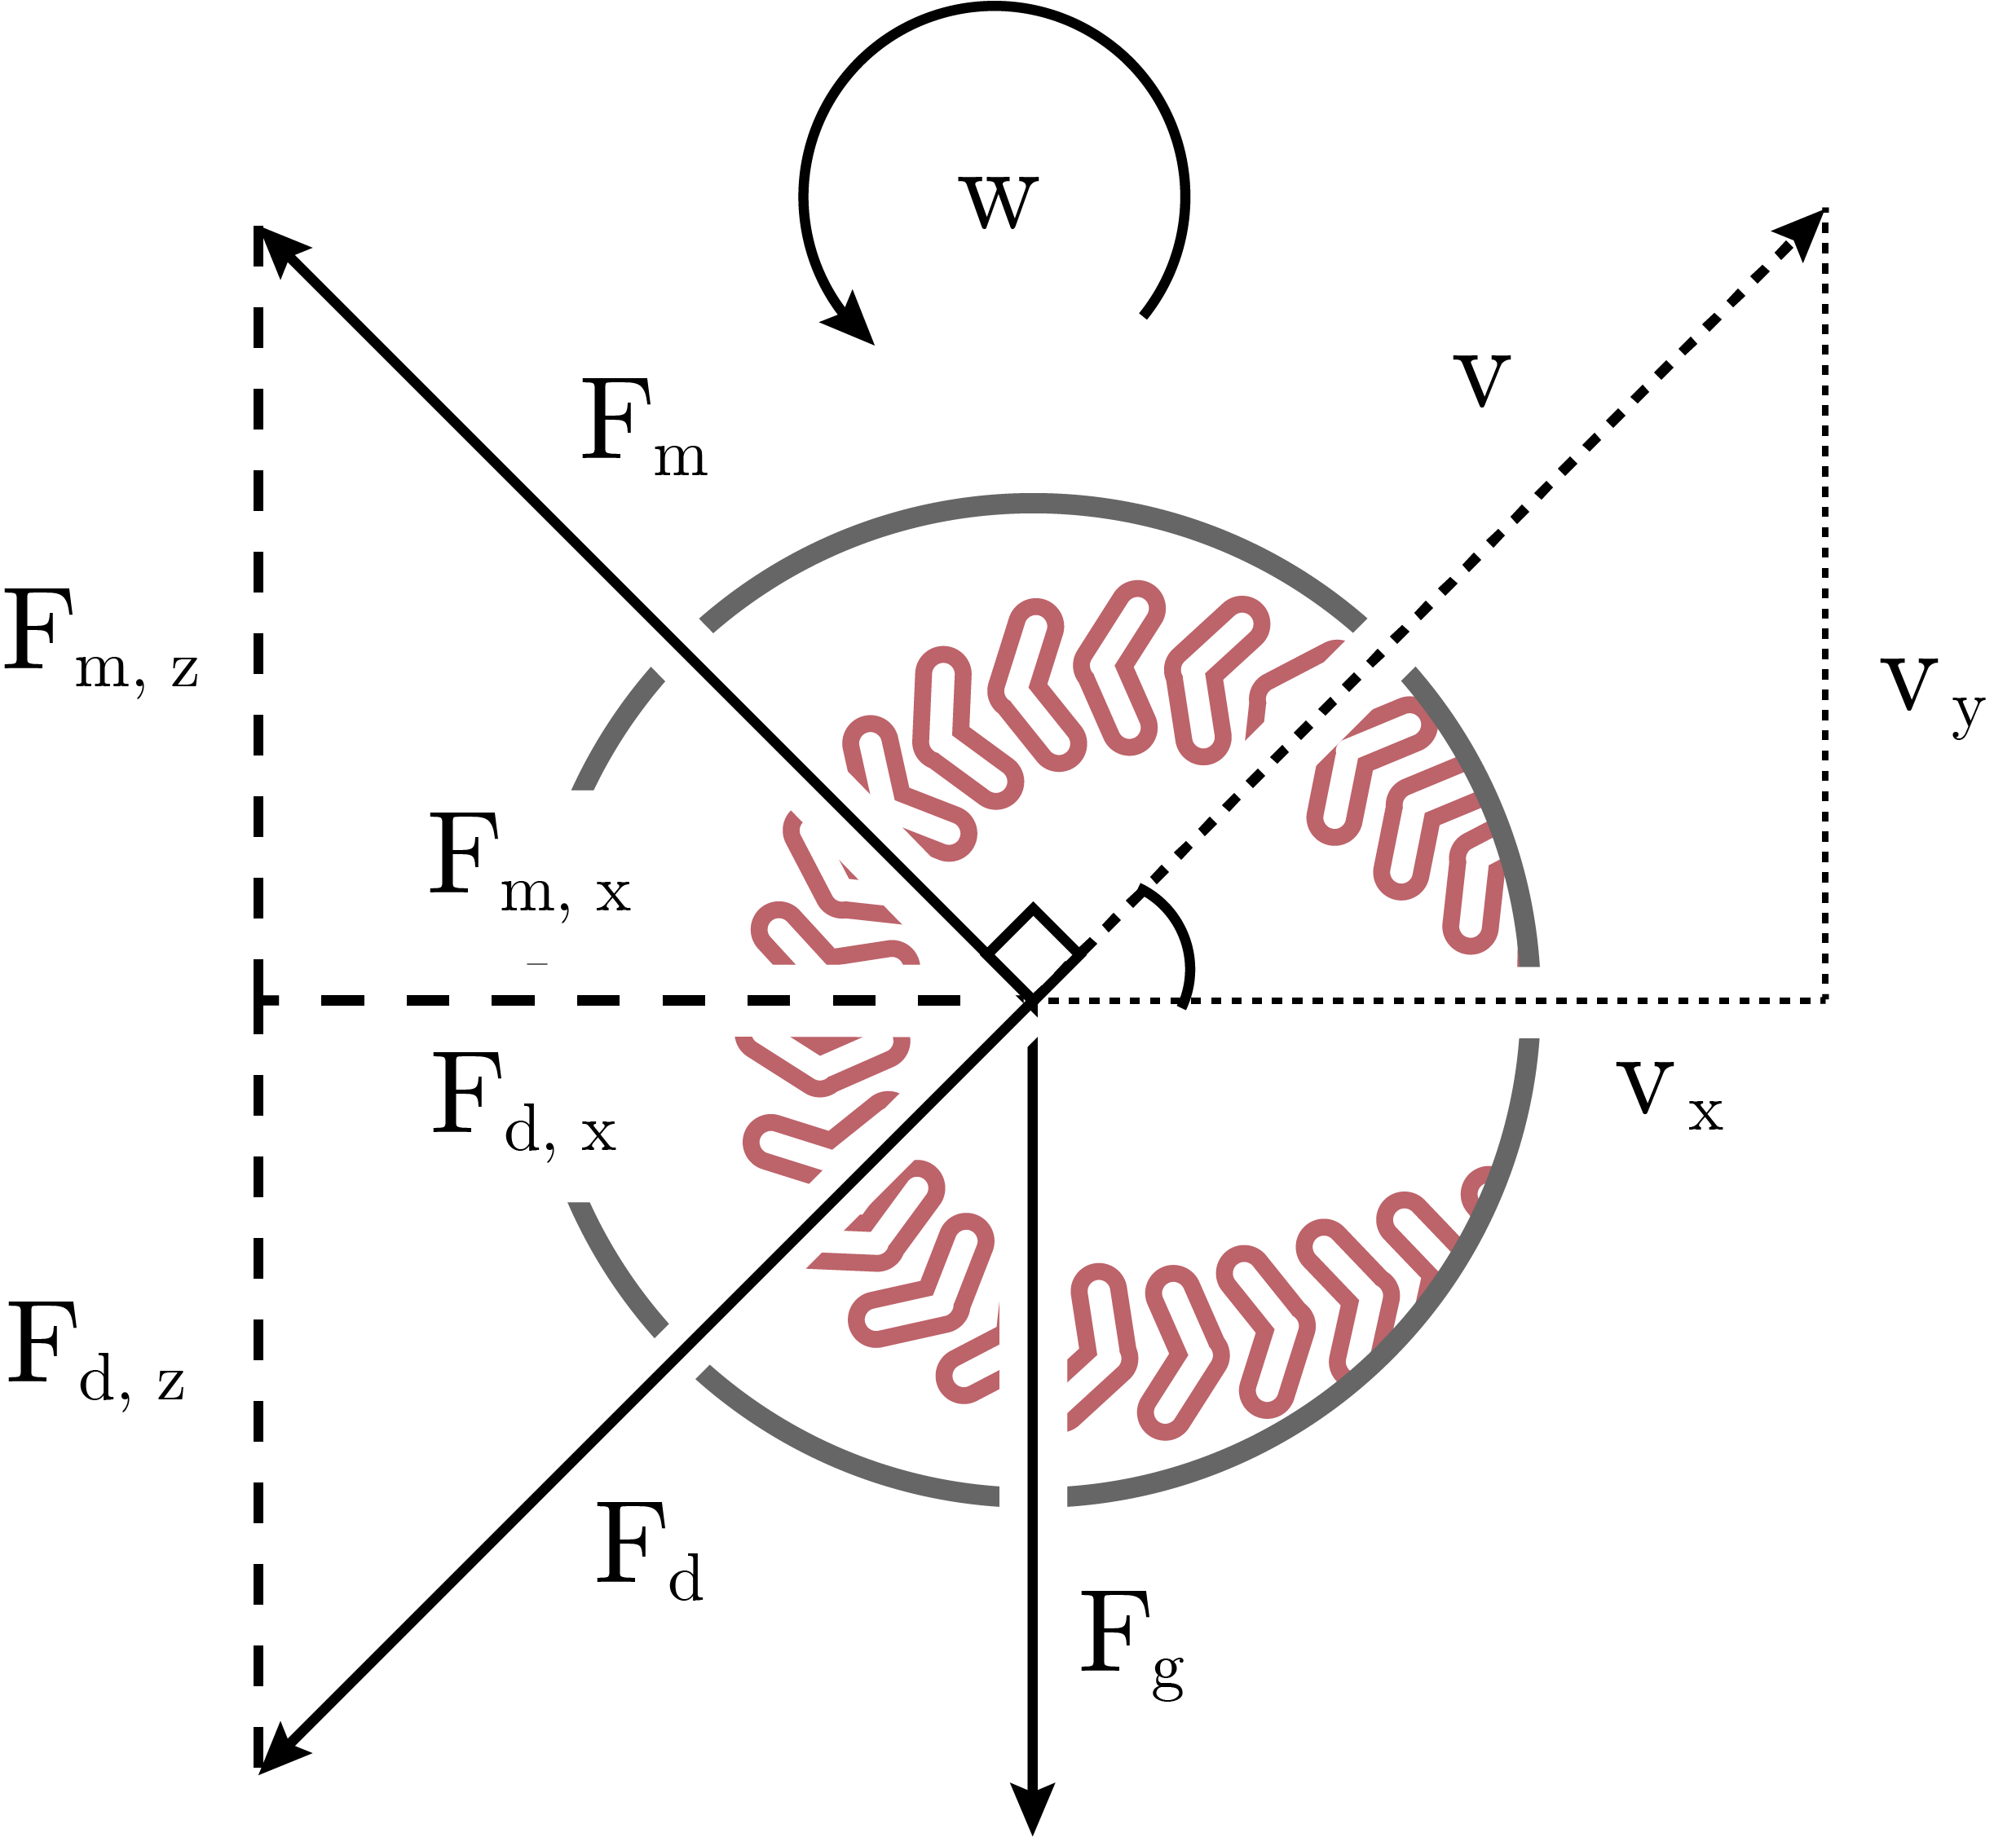
\includegraphics[width=\linewidth]{figures/forces.png}
    \caption{A free-body diagram of a baseball in-flight illustrating the three main forces influencing the ball's trajectory through x-z space. The magnitudes are not to scale. The ball's direction of motion is at an angle of 45$^\circ$ $(\pi/4$ rad) from parallel with the ground with pure backspin. The optimal angle is actually shallower, between 20 and 30 degrees. The spin axis is usually not purely in the y dimension (in or out of the screen), however, in the absence of real spin axis data, this is a decent assumption. ``w'' is standing for $\omega$ here because I haven't figured out how to type Greek letters in Photoshop yet.}\label{fig:forces}
\end{figure}

\subsection{Atmosphere Effects}

For the second question I can find the average drag on the ball for each MLB stadium by calculating the air density based on \texttt{open-mateo} data and the ideal gas physics then numerically calculate a trajectory through x-z space using Euler's Method. There are three main forces that influence the trajectory of a ball: gravity, drag, and the Magnus force. Fig~\ref{fig:forces} shows and ideal example free-body diagram of these forces and the direction of motion. These forces are described parametrically in~\cite{adair2002},~\cite{Sawicki2003}, and~\cite{Nathan2008_spin} as
\begin{equation}
    F_g = -mg
\end{equation}
\begin{equation}
    F_d = \frac{1}{2}C_d\rho A v^2
\end{equation}
\begin{equation}
    F_m = \frac{1}{2}C_l\rho A v^2
\end{equation}

where $m$ is the mass of the ball, $g$ is the acceleration due to gravity, $v$ is the velocity vector, $\rho$ is the air density, $A$ is the cross-sectional area of the ball, $C_d$ is the drag coefficient, and $C_l$ is the lift coefficient. The drag and lift coefficients for an MLB baseball were experimentally determined in~\cite{Sawicki2003} and~\cite{Nathan2008_spin} as

\begin{equation}
    C_l = \begin{cases}
        0.09 + (0.6  S) \text{ if } S>0.1\\
        1.5S \text{ if } S\le0.1
    \end{cases}
\end{equation}
\begin{equation}
    C_d = 0.3 + 0.03 S
\end{equation}

where $S = R \omega/ v$. The radius and mass of an MLB baseball are also well established; I will use $R = 0.0364$m and $m = 0.145$kg. $F_d$ and $F_m$ depend on $\omega$ and $v$ in addition to $R$ which will be input parameters to the model (hit variables). This leave just the air density which I can estimate using the ideal gas law
\begin{equation}
    PV = nRT \rightarrow n/V = \rho = P/RT 
\end{equation}
where $P$ is pressure (Pa), $V$ is volume (m$^3$), $n$ is the number of moles, $R$ is the ideal gas constant ($\rm J\cdot mol^{-1}\cdot K^{-1}$), and $T$ is the temperature (K), and $\rho$ is the air density ($\rm mol\cdot m^{-3}$). This equation will yeild the number density of moles of air particles per cubic meter which I can convert to a mass denisty (which the above models expect) by multiplying the number density by the mass of dry air $m_{\rm air} = 0.0289647$ $\rm kg \cdot mol^{-1}$. To get pressure I can pull elevation data from \texttt{open-mateo} using stadium coordinate data. The elevation can translate to pressure via barometric formula.
\begin{equation}
    P = P_0 (1 - 2.25577 \cdot 10^{-5} \cdot e)^{5.25588}
\end{equation}
where $P_0 = 101325$ Pa is the pressure at sea level, and $e$ is the elevation (m). This leave just the temperature unresolved. For this I can pull hourly temperature data from \texttt{open-mateo} from the start time of each game during the 2025 MLB season for each team to find the average air density during a given game at each current MLB stadium. All together, I can combine equations 1-7 with Euler's Method to numerically calculate a trajectory for a given set of hit parameters ($v$, $\omega$, $\theta_{\rm angle}$ (launch angle), and $\theta_{\rm axis}$ (spin axis)) for the average game at each current MLB stadium.

\subsection{Competitive Advantages}

For the third question I look at if there has been any major competitive impact to Mariners players or seasons based on player archetype. This question is specifically motivate by this year's team which is built as a ``slugging'' team which some criticize for a place like Seattle for not playing into the strengths of the park. The New York Yankees, for example, tend to buy or trade for left handed power hitters because right field in Yankee Stadium is significantly shorter than in other parks, turning pop-outs into home-runs for 81 games a year. I will look at the top and bottom offensive WAR (Wins Above Replacement, used to evaluate a player's overall worth) Mariners players in a single season at home over the past 10 years and inspect their play-style. I will compare home-runs, batting average, average launch angle, average exit velocity, and maybe a few more things. I will use this to draw a conclusion about what play-styles are most effective in T-mobile Park, or if there is a trend at all.

\section{EDA Results}

For the EDA I built one of the functions for question 1: how does player performance change when traded to or from the Mariners? I also made significant progress on question 2: does the air density, wind, temperature, and/or humidity in Seattle cause baseballs to travel differently compared to other major league stadiums and is it disadvantageous to hitters?

\subsection{Question 1}
I attacked this one first because seemed the hardest to implement. To do this, I used the \texttt{batting\_stats\_bref} function from \texttt{pybaseball} which takes a year argument and returns a DataFrame of all of the batting statistics for that season (seasons lineup with calendar years in MLB baseball). Each row is a unique player with the headers

\begin{verbatim}
'Name', 'Age', '#days', 'Lev', 'Tm',
'G', 'PA', 'AB', 'R', 'H', '2B', '3B',
'HR', 'RBI', 'BB', 'IBB', 'SO', 'HBP',
'SH', 'SF', 'GDP', 'SB', 'CS', 'BA',
'OBP', 'SLG', 'OPS', 'mlbID'
\end{verbatim}

For my function, I wanted the inputs to be a team (actually a location of a team because the \texttt{'Tm'} parameter returns \texttt{'Seattle'} for Mariner players for example), as well as a range of seasons which will default to all the available data if not specified (2008 -- 2026). I also wanted an optional minimum plate appearances or at-bats so that players who only played a small amount can be filtered out. The output from this file is shown in Fig~\ref{fig:seaborn}.

\begin{figure}
    \centering
    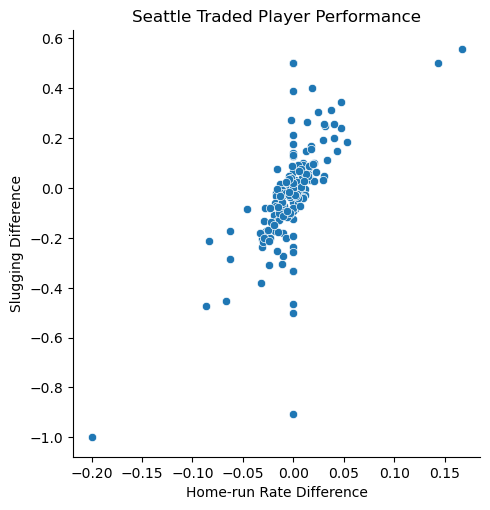
\includegraphics[width=\linewidth]{figures/Seattle_traded_player_performance.png}
    \caption{The change in performance of all players traded to or from the Seattle Mariners between 2008 and 2026 in the seasons on either side of the trade. Negative values indicate worse performance as a Mariner and vice versa. There are no cuts for minimum play (AB or PA).}
    \label{fig:seaborn}
\end{figure}

According to some papers on baseball statistics, each of these metrics has a critical number of plate appearances or at-bats before they become statistically significant. As a part of this I have been reading from Slowinski (2010) and Pemstein (2015) which look at Cronbach's alpha and $R^2$ for determining a minimum sample size for each of these stats to be `trustable'.

\subsection{Question 2}

Using the equations described in Sec 4.2, I built the numerical calculator that traces a ball's trajectory in x-z space. This time-stepping scheme is a very classing structure to follow in Physics models. It is commonly called Euler's Method which you can read about it you'd like. The basic idea is at each timestep, you take the conditions from the previous step (like position and velocity) and apply the forces to the object based on those conditions, updating them for the next time step. When the time steps are small enough, you can trace out smooth arcs like how a baseball travels through the air. Any undergraduate physicist will have done this at some point, the challenge here was just moving it to Python. The output plot from main is shown in Fig~\ref{fig:trajectories} with some fun environments that test the extremes. 

during the EDA I was worried about the effect of spin-down on the ball as friction with the air causes the ball so slow its angular velocity, however, \citep{Nathan2008_spindown} suggests this effect will be trivial in all real-world conditions.

\begin{figure}
    \centering
    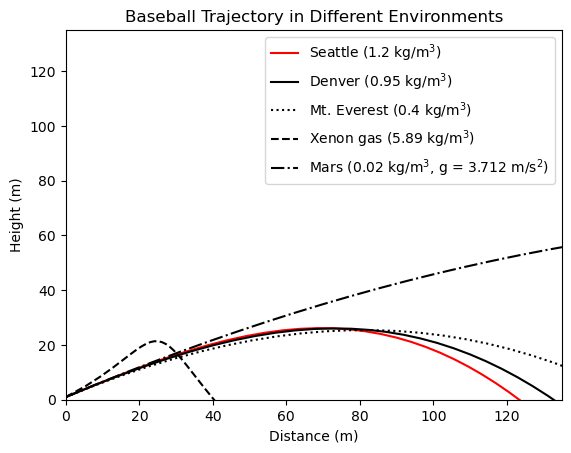
\includegraphics[width=\linewidth]{figures/trajectory_plot.png}
    \caption{The trajectory of a baseball hit at 45$\rm m/s$ at an angle of $\pi/4$ rad (45$^\circ$) with pure backspin and a spin rate of 150 rad/s ($\approx$ 1,500 rpm) in different environments. The environmental data on air density each came from a quick google search but will eventually be replaced by a calculated air density based on the elevation and temperature data from my second dataset. I'm going to need to figure out how to force the axes to be the same scale so that the angle representation isn't skewed like it is here.}
    \label{fig:trajectories}
\end{figure}

\section{Results}

\subsection{Historical Batting}

The stats I chose to look at for batting statistics were 1B rate (single rate), OBP, HR rate, and SLG. I had initially planned on using batting average as well but~\cite{slowinski2010} suggests that this stat requires a very large sample size to converge to statistically significant, 920 plate appearances (PA) to be exact which is way too big to be usefull for any of the analysis I'm doing here. Instead I focused on OBP (460 PA), 1B rate (290 PA), HR rate (170 PA), SLG (320 AB). For the traded player stats, single rate did not end up being easily calculable and was not worth re-adding considereing the results.

\begin{figure*}
    \centering
    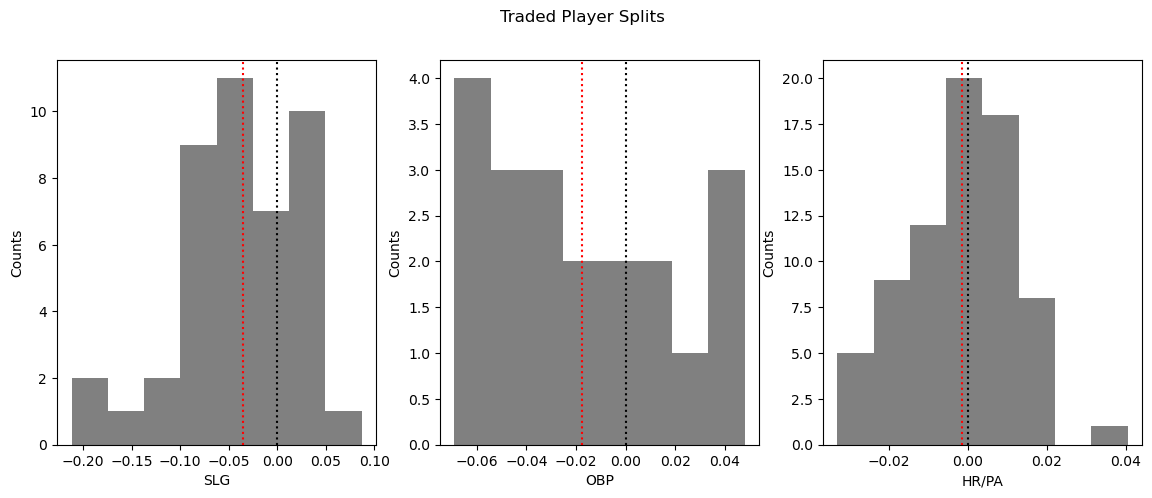
\includegraphics[width=\linewidth]{figures/traded_player_performance.png}
    \caption{The statistical splits for OBP, HR rate, and SLG for traded players between 2008 and 2025. More Negative indicates a worse performance as a Mariner.}\label{fig:traded_player}
\end{figure*}

There was little to no difference in overall hitting splits for players traded to or from the Mariners for OBP, HR rate, and SLG. Additionally, the samples sizes were too small to resemble a clean gaussian distribution, indicating that they are not statistically significant at this scale. This can be seen in Fig~\ref{fig:traded_player}. HR rate, which had the lowest minimum PA threshold, does resemple a gaussian distribution with 20 counts at the peak but deviates by less than 0.5\% from 0. This suggests no overall effect on player's home-run rates when changing home fields to or from T-Mobile Park.

There was also little to no difference when comparing home or away splits for Mariner hitters. These sample sizes were much larger and produced much more gaussian distributions, however, while the splits for three of the four tracked stats were negative, they deviated from zero only $\sim 3\%$ at the most. HR rate did not deviate. This is shown in Fig~\ref{fig:home_away}

\begin{figure*}
    \centering
    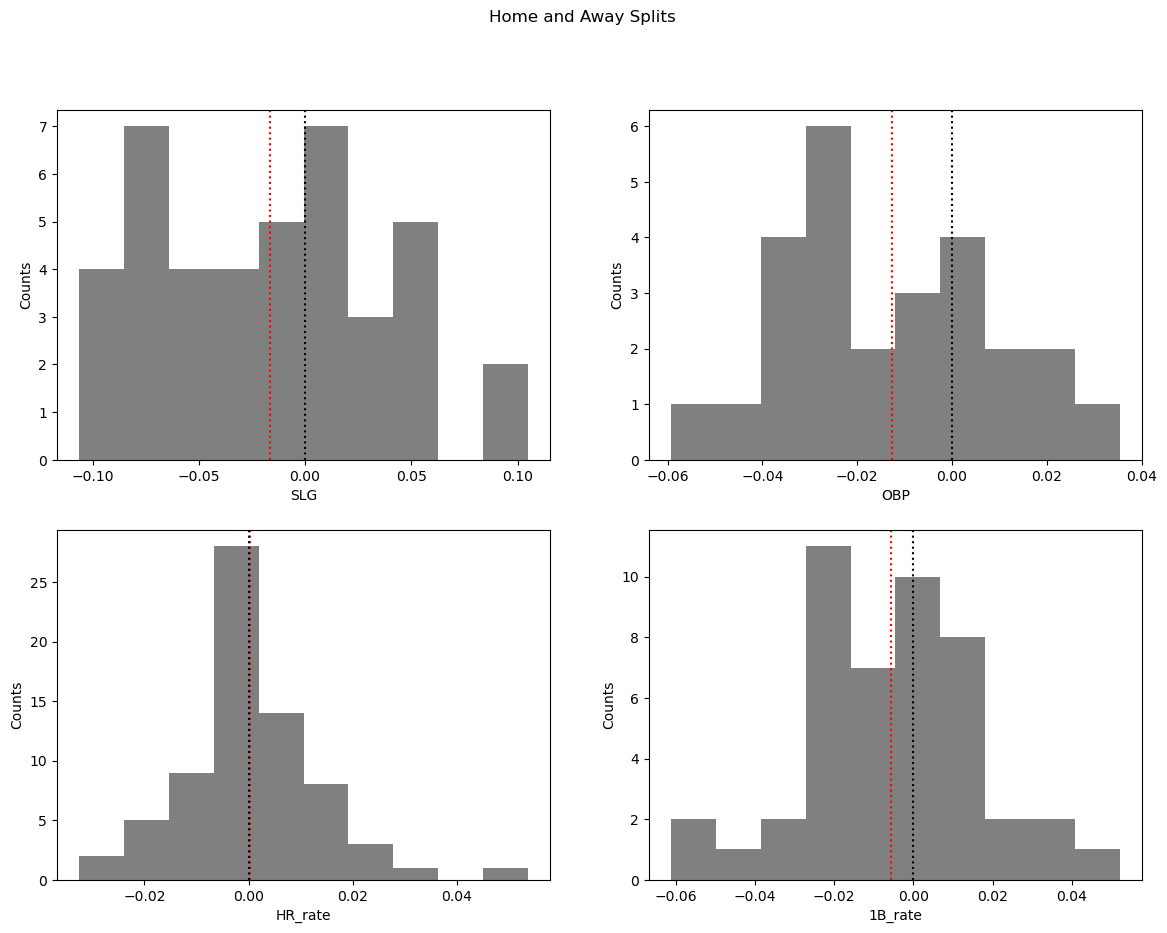
\includegraphics[width=\linewidth]{figures/home_away_splits.png}
    \caption{The home and away splits for OBP, HR rate, single rate, and SLG for Mariner players between 2008 and 2025. More Negative indicates a worse performance at home.}\label{fig:home_away}
\end{figure*}

\subsection{Atmosphere Effects}

\subsection{Competitive Disadvantages}

\section{Impact and Limitations}

These results from question 1 show little systematic production changes sue to players playing in Seattle or for the Mariners. This would suggest that the poor team perfromances are due to errors in recruiting and player evaluation by the organization. It also could suggest that perhaps Mariner teams simply use capital in areas besides hitting. The results from question 2 show that hard-hit, high-angle balls do not result in as far trajectories in Seattle compared to other stadiums. This would suggest that sluggers who rely on home-runs for run production likely aren't the best fit for a team playing in Seattle for half of thier games. This is a particularly important implication given the current team's reliance on home-runs. There are clear limitations to this analysis. The most pressing are the feild dimensions which weren't accounted for here and the assumptions about spin rate on batted balls which is not publicly tracked.

\section{Challenge Goals}
My challenge goals have been a bit of a mess because I am doing a lot of things that could be a challenge goal. In the end I used multiple datasets and used a second library. I used \texttt{open-mateo} and the small manually entered \texttt{stadium\_data.csv} for the weather and elevation data in combination with the trajectory calculator function.

\section{Work Plan Evaluation}
I followed my work plan almost exactly. 

\begin{enumerate}
    \item Install and figure out \texttt{pybaseball} indexing and manipulation $\checkmark$
    \item Build function for Euler's Method trajectory calculator and main method $\checkmark$
    \item Build function and main method for traded player stats $\checkmark$
    \item Build function for pulling weather data from \texttt{open-mateo} to use in trajectory calculator function $\checkmark$
    \item Build function and main method for home/away hitting splits $\checkmark$
    \item Go back and produce any more visualizations I will need $\checkmark$
    \item Write docs for each function using mark-down $\checkmark$
    \item Write-up findings in \LaTeX $\checkmark$
\end{enumerate}
I also have and will continue to push my project to GitHub.

\section{Testing}

\bibliographystyle{apalike}
\bibliography{ref}

\end{document}